\chapter{Specific Requirements} \label{specificRequirements}

\section{External Interfaces}

\begin{figure}[H]
    \centering
    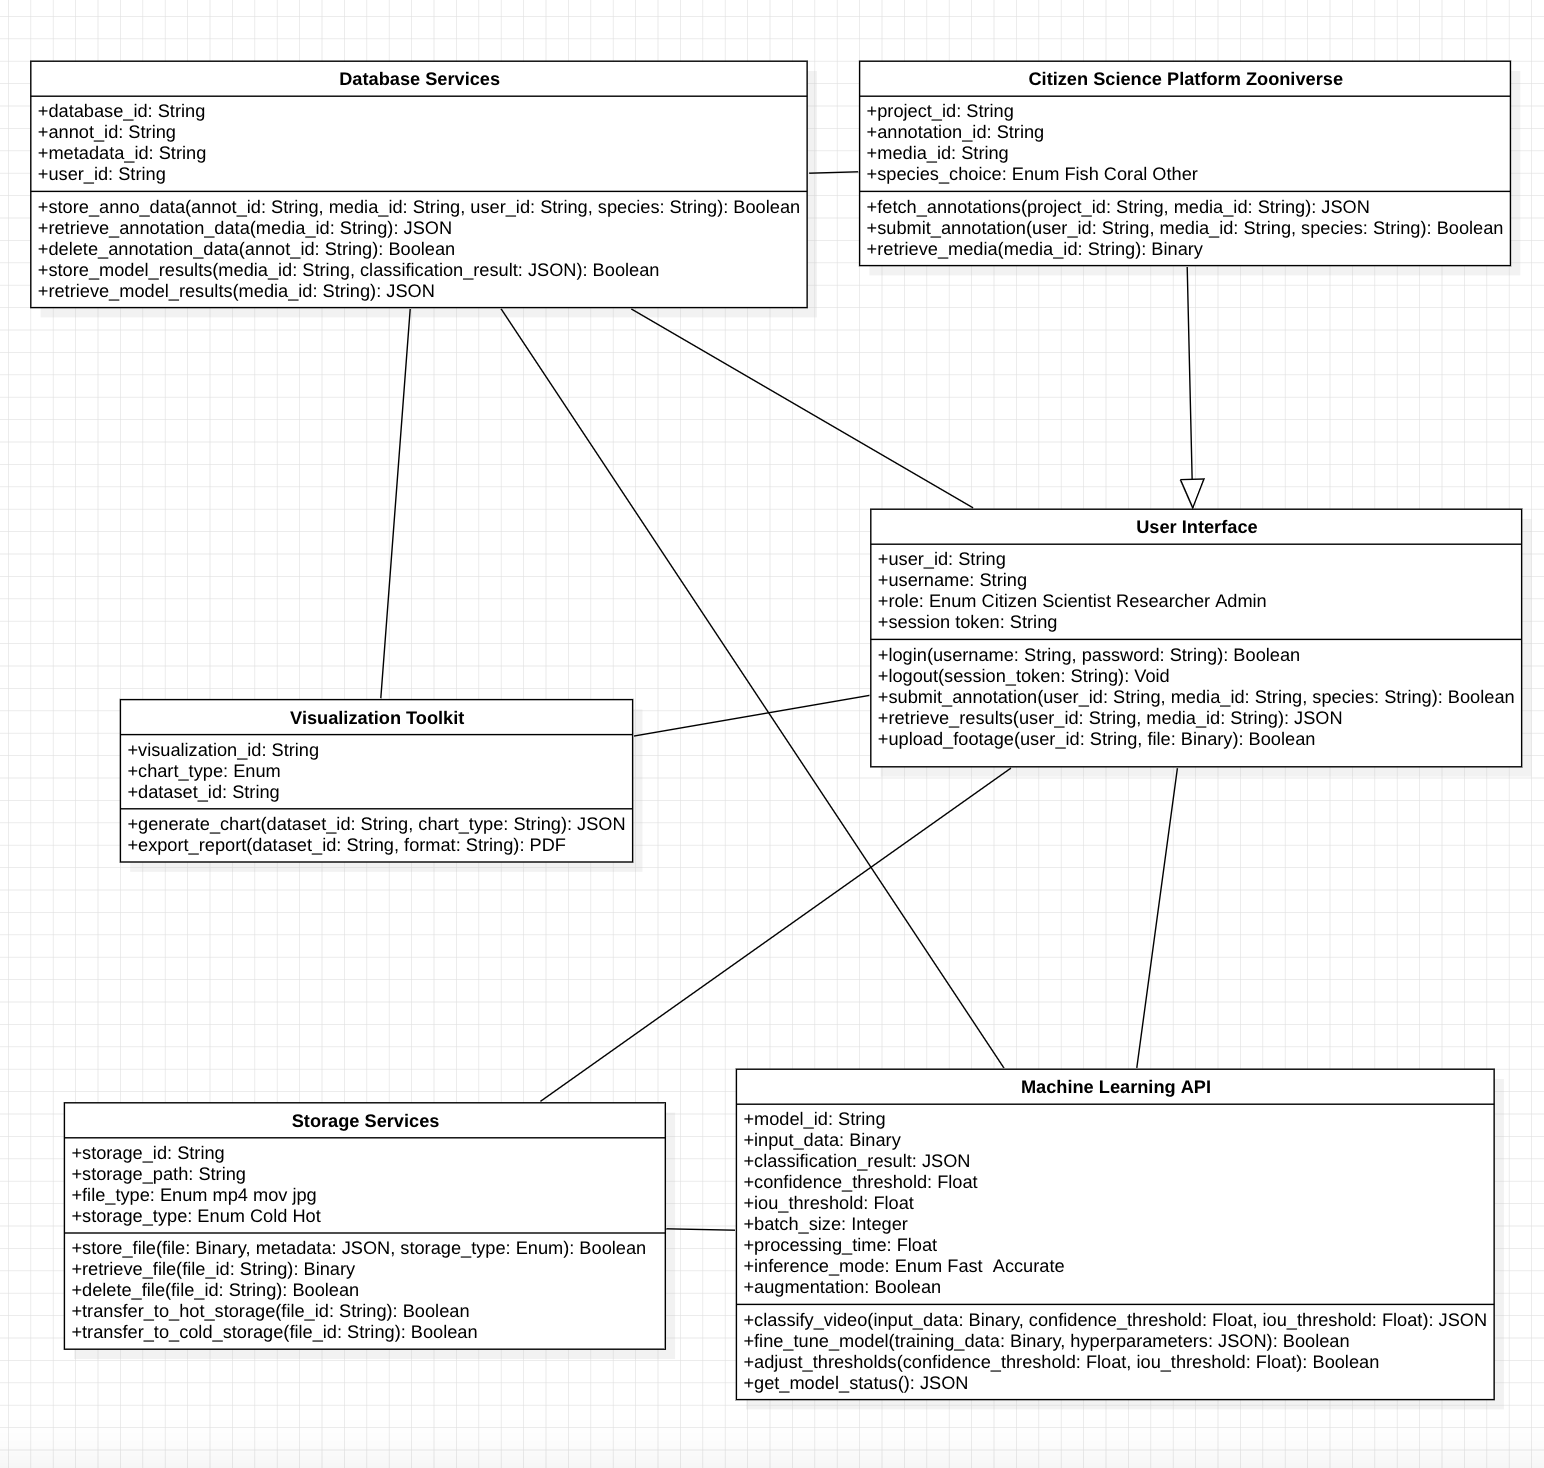
\includegraphics[width=1 \textwidth]{Figures/ExternalInterfaces.png}
    \caption{External Interfaces Diagram \label{Fig:External Interfaces Diagram}}
\end{figure}

The \textbf{User Interface} allows citizen scientists and researchers to interact with the system via a web platform or API, enabling annotation submission, footage uploads, and result retrieval.

The \textbf{Citizen Science Platform} enables volunteers to classify marine species in videos via Zooniverse, aggregating multiple annotations to improve accuracy.

The \textbf{Machine Learning API} processes video footage using AI models like TensorFlow and YOLOv3, providing automated species classification with configurable thresholds.

The \textbf{Storage Service} manages video and image files, with cold storage for long-term archival and hot storage for frequently accessed data used in annotation and ML processing.

The \textbf{Database Service} stores metadata, species classifications, and annotations, ensuring structured data management and interoperability with storage and ML components.

The \textbf{Visualization Toolkit} provides interactive graphical tools for researchers to analyze and validate classification results, generate reports, and fine-tune model parameters.


\section{Functions}

\begin{figure}[H]
    \centering
    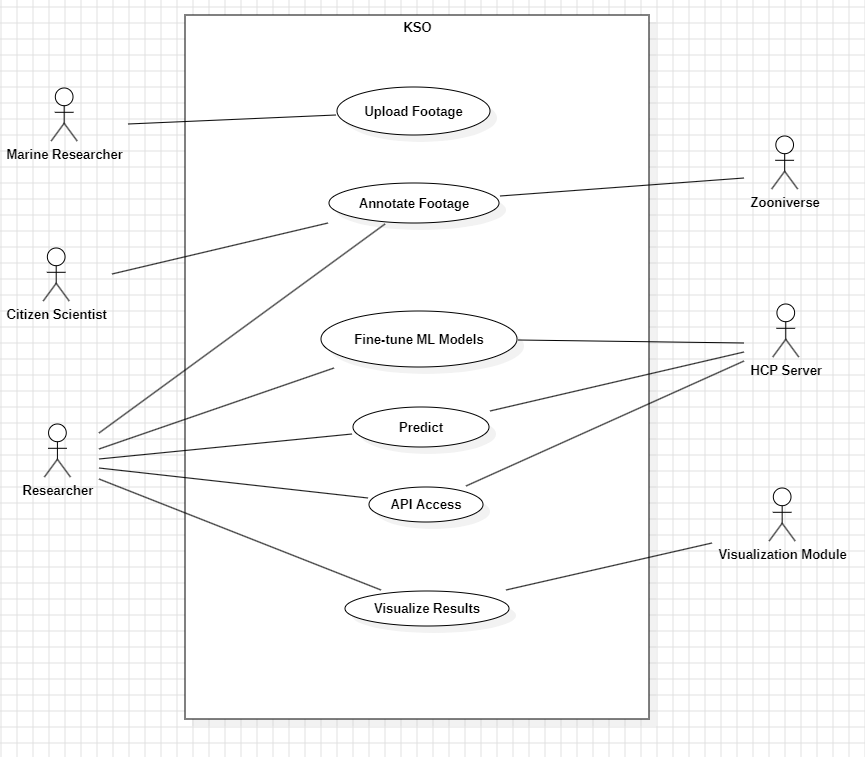
\includegraphics[width=1 \textwidth]{Figures/UseCase Diagram.png}
    \caption{Use Case Diagram \label{Fig:Use Case Diagram}}
\end{figure}

\begin{table}[H] 
    \centering
    \small
    \begin{tabularx}{\textwidth}{|>{\bfseries\hsize=.5\hsize\linewidth=\hsize}X|
    >{\hsize=1.5\hsize\linewidth=\hsize}X|}
    \hline
    Use Case Name       & Upload Underwater Footage to KSO \\ \hline
    
    Actors              & Marine Researcher \\ \hline
    
    Description         & A Marine Researcher uploads long ROV/AUV movie files to the system, 
    which are archived in cold storage and optionally transferred to hot 
    storage for frequent processing.  \\ \hline
    
    Pre-Conditions      & 
    - Researcher has valid KSO credentials.\newline
    - Network connection is stable.\newline
    - Adequate storage is available. \\ \hline
    
    Data                & 
    - ROV/AUV video files (1--2 hours each).\newline
    - Associated metadata (timestamp, location, etc.). \\ \hline
    
    Response            & 
    - Files are archived.\newline
    - Confirmation returned to the researcher.\newline
    - Metadata recorded in the KSO database. \\ \hline
    
    Stimulus            & Researcher initiates the ``Upload Footage'' action. \\ \hline
    
    Normal Flow         & 
    1. Researcher logs into the KSO interface.\newline
    2. Researcher selects ``Upload Footage'' and provides files/metadata.\newline
    3. System validates file format and storage availability.\newline
    4. System saves files to cold storage and logs metadata.\newline
    5. System confirms successful upload to the researcher. \\ \hline
    
    Alternative Flow    & If immediate analysis is needed, the system also copies files to hot storage. \\ \hline
    
    Exception Flow      & 
    - \textbf{File Validation Error:} The system rejects incompatible/corrupted files.\newline
    - \textbf{Insufficient Storage:} The system notifies the researcher and aborts the upload. \\ \hline
    
    Post-Conditions     & 
    - Footage and metadata are successfully stored and discoverable in the KSO. \\ \hline
    
    Comments            & 
    - May be extended by a metadata-management sub-process if additional edits are required. \\ \hline
    \end{tabularx}
    \caption{Tabular Description of \textit{Upload Underwater Footage to KSO} \label{Tab:UseCase1}}
    \end{table}

        \begin{table}[H] 
            \centering
            \small
            \begin{tabularx}{\textwidth}{|>{\bfseries\hsize=.5\hsize\linewidth=\hsize}X|
            >{\hsize=1.5\hsize\linewidth=\hsize}X|}
            \hline
            Use Case Name       & Annotate Footage via Citizen Science \\ \hline
            
            Actors              & Citizen Scientist, Zooniverse, Researcher \\ \hline
            
            Description         & 
            Citizen Scientists watch the 10-second clips and identify which species (if any) 
            appear, possibly entering count information and timestamps. The aggregated 
            results are pulled into KSO. \\ \hline
            
            Pre-Conditions      & 
            - Clips should have been uploaded to Zooniverse.\newline
            - Species choices and instructions are configured.\newline
            - Citizen Scientist has access to the project. \\ \hline
            
            Data                & 
            - 10-second video clips.\newline
            - Species/label lists. \\ \hline
            
            Response            & 
            - Annotation responses recorded in Zooniverse.\newline
            - Each clip is retired once enough classifications are gathered. \\ \hline
            
            Stimulus            & 
            Citizen Scientist visits the Koster Seafloor Observatory project in Zooniverse 
            and requests a new clip to classify. \\ \hline
            
            Normal Flow         & 
            1. Citizen Scientist logs in (or continues anonymously, if allowed).\newline
            2. Zooniverse serves a 10-second clip.\newline
            3. Citizen Scientist selects species, counts, and timestamps.\newline
            4. Classification is submitted and stored.\newline
            5. Once the clip meets the required number of classifications, it is retired.\newline
            6. Aggregated data is periodically transferred to KSO. \\ \hline
            
            Alternative Flow    & 
            - Multiple species can be selected per clip.\newline
            - ``Unsure'' or ``Nothing here'' can be chosen for ambiguous clips. \\ \hline
            
            Exception Flow      & 
            - \textbf{Platform Unavailable:} Classification cannot proceed.\newline
            - \textbf{Network Timeout:} Submitted data may be lost if the session disconnects. \\ \hline
            
            Post-Conditions     & 
            - Citizen Scientist input is used for consensus labeling in KSO’s data module. \\ \hline
            
            Comments            & 
            - This includes or precedes the aggregation of classifications (see Use Case 4). \\ \hline
            \end{tabularx}
            \caption{Tabular Description of \textit{Annotate Footage via Citizen Science} \label{Tab:UseCase2}}
            \end{table}
            \begin{figure}[H]
                \centering
                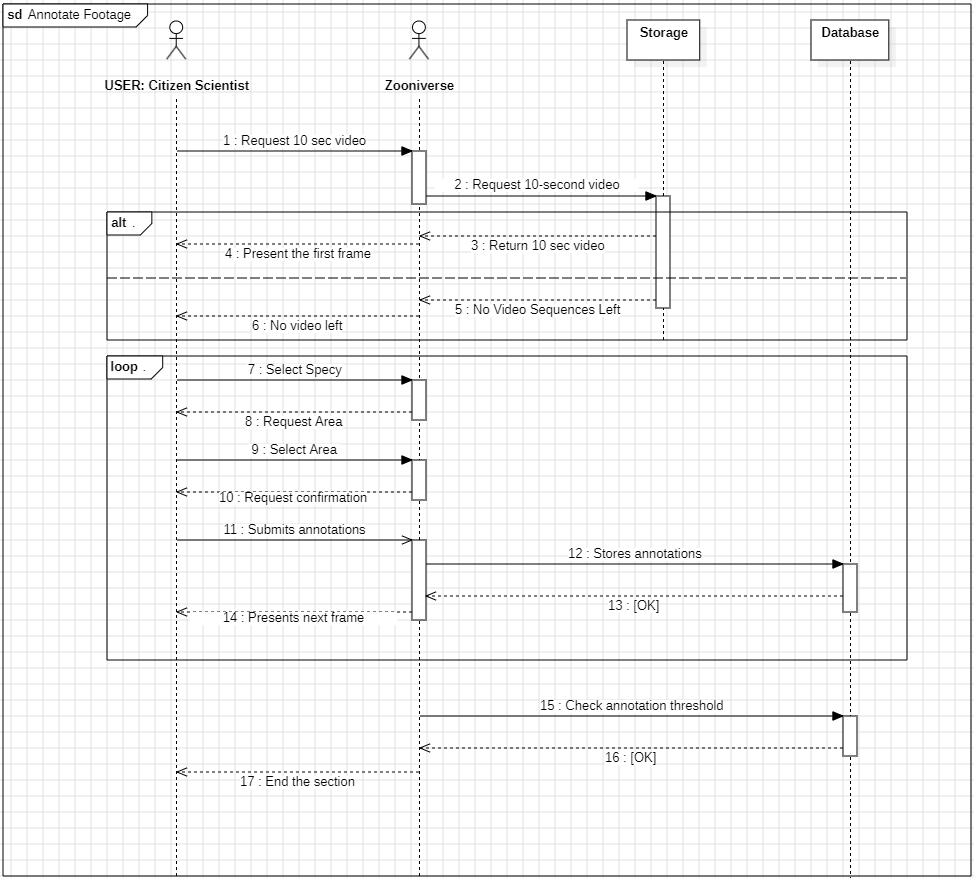
\includegraphics[width=1 \textwidth]{Figures/Sequence Diagram.png}
                \caption{Sequence Diagram for Annotate Footage \label{Fig:Sequence Diagram}}
            \end{figure}
            \begin{table}[H] 
                \centering
                \footnotesize
                \begin{tabularx}{\textwidth}{|>{\bfseries\hsize=.5\hsize\linewidth=\hsize}X|
                >{\hsize=1.5\hsize\linewidth=\hsize}X|}
                \hline
                Use Case Name       & Fine-tune Machine Learning Models \\ \hline
                
                Actors              & Researcher, HPC Server \\ \hline
                
                Description         & 
                Fine-tune machine learning models using citizen scientist-annotated data for automated species detection in subsea footage. \\ \hline
                
                Pre-Conditions      & 
                - Annotated datasets ready and validated; machine learning infrastructure available. \\ \hline
                
                Data                & 
                - Annotated video/image datasets \newline 
                - Data augmentation scripts preprocessing tools \newline
                - Machine learning scripts \\ \hline
                
                Response            & 
                - Machine learning model fine-tuned, validated, and available for further application. \\ \hline
                
                Stimulus            & 
                Researcher initiates the ML model fine-tuning process. \\ \hline
                
                Normal Flow         & 
                1. The Researcher uploads the annotated subsea imagery dataset along with fine-tuning parameters (epochs, learning rate, early stopping, confidence thresholds).\newline
                2. The KSO API validates the dataset and parameter integrity, confirming they meet the required standards.\newline
                3. The HPC Server iteratively trains and validates the machine learning model, monitoring performance metrics until the defined epochs are completed or early stopping criteria are met.\newline
                4. Upon completion, the HPC Server evaluates performance metrics (F1-score, precision, recall, mAP) and securely stores the trained model.\newline
                5. The Researcher reviews the fine-tuning outcomes and either accepts the results or revisits parameters for further iterations, returning to step 2 if necessary.\\ \hline
                
                Alternative Flow    & 
                - Researcher modifies hyperparameters and re-tunes the model based on initial evaluation metrics. \\ \hline
                
                Exception Flow      & 
                - If computational resources are insufficient or there are script errors, training halts, and the issue is logged and reported to the system administrator. \\ \hline
                
                Post-Conditions     & 
                - Machine learning model is accurately tuned, validated, and ready to predict ecological observations from new footage. \\ \hline
                
                Comments            & 
                - Ensuring data quality and appropriate parameter tuning are critical for the accuracy and reliability of the tuned model. \\ \hline
                \end{tabularx}
                \caption{Tabular Description of \textit{Fine-tune Machine Learning Models} \label{Tab:UseCase2}}
                \end{table}
                \begin{figure}[H]
                    \centering
                    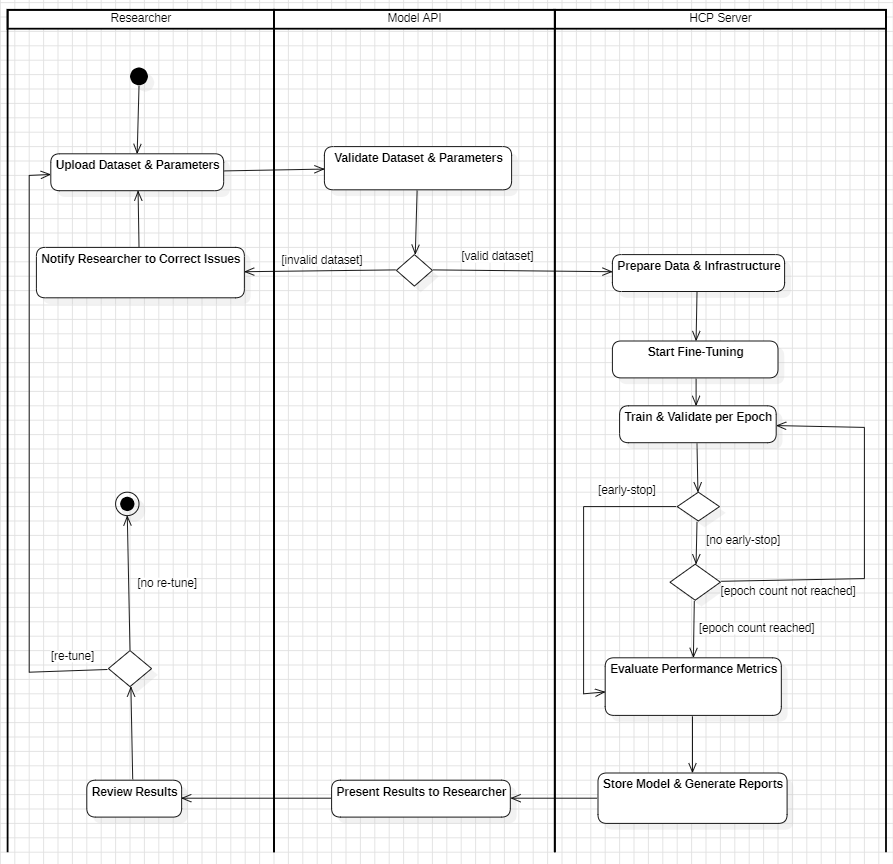
\includegraphics[width=1 \textwidth]{Figures/Activity Diagram.png}
                    \caption{Activity Diagram of Fine-tuning ML Models\label{Fig:Activity Diagram}}
                \end{figure}

            \begin{table}[H] 
                \centering
                \small
                \begin{tabularx}{\textwidth}{|>{\bfseries\hsize=.5\hsize\linewidth=\hsize}X|
                >{\hsize=1.5\hsize\linewidth=\hsize}X|}
                \hline
                Use Case Name       & Running Predictions on New Footage \\ \hline
                
                Actors              & 
                Researcher, HPC Server \\ \hline
                
                Description         & 
                The trained model is used to detect target species in newly uploaded or 
                unseen footage, generating bounding boxes and presence/absence data. \\ \hline
                
                Pre-Conditions      & 
                - A trained model is available.\newline
                - Inference thresholds (confidence, IOU) are set. \\ \hline
                
                Data                & 
                - Model weights.\newline
                - New video/image frames.\newline
                - Inference parameters. \\ \hline
                
                Response            & 
                - Detected bounding boxes with confidence scores.\newline
                - Presence/absence data logged in the KSO database. \\ \hline
                
                Stimulus            & 
                Researcher selects ``Analyze New Footage'' or calls the ML API. \\ \hline
                
                Normal Flow         & 
                1. Researcher chooses which footage to process.\newline
                2. System loads the model and HPC resources.\newline
                3. Model runs inference per frame/clip, generating bounding boxes.\newline
                4. Consecutive bounding boxes are combined if necessary (e.g., continuous detection).\newline
                5. Results are returned to the researcher. \\ \hline
                
                Alternative Flow    & 
                Researcher adjusts confidence or IOU thresholds, re-runs inference to 
                fine-tune detection results. \\ \hline
                
                Exception Flow      & 
                - \textbf{Model Version Missing:} The system prompts user for a valid model.\newline
                - \textbf{HPC Failure:} Job is interrupted; system logs error and notifies researcher. \\ \hline
                
                Post-Conditions     & 
                - Updated detection data is stored for subsequent mapping or 
                  time-series analysis.\newline
                - The KSO can render distribution maps or other summaries. \\ \hline
                
                Comments            & 
                - Often extended by a "Visualize and Report Biodiversity Data" use case for output data. \\ \hline
                \end{tabularx}
                \caption{Tabular Description of \textit{Running Predictions on New Footage} \label{Tab:UseCase3}}
                \end{table}
                

                \begin{figure}[H]
                    \centering
                    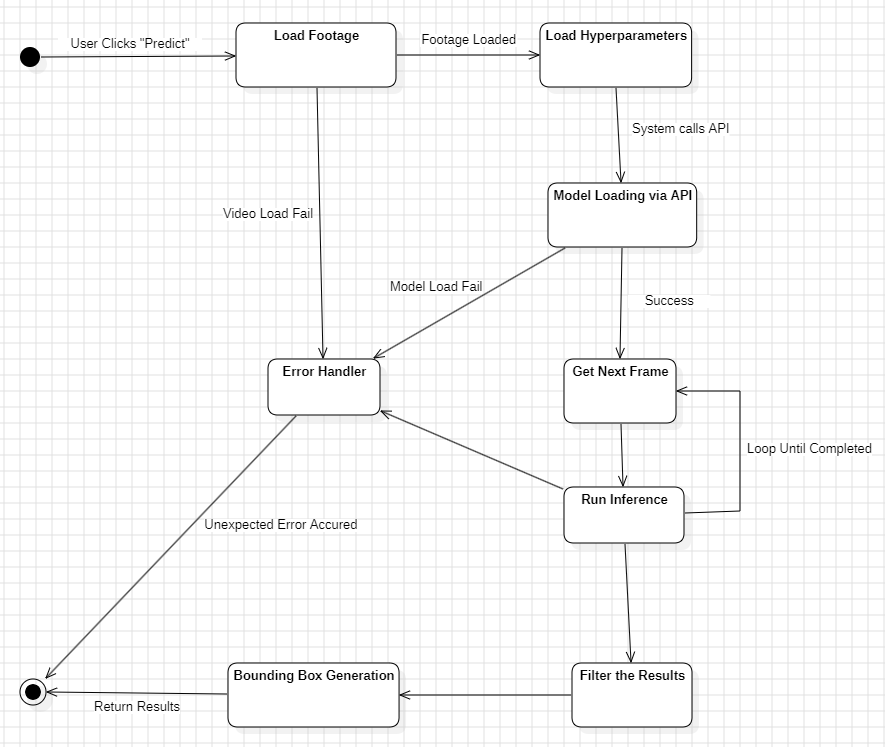
\includegraphics[width=1 \textwidth]{Figures/State Diagram.png}
                    \caption{State Diagram of Running Predictions\label{Fig:State Diagram}}
                \end{figure}

                \begin{table}[H] 
                    \centering
                    \small
                    \begin{tabularx}{\textwidth}{|>{\bfseries\hsize=.5\hsize\linewidth=\hsize}X|
                    >{\hsize=1.5\hsize\linewidth=\hsize}X|}
                    \hline
                    Use Case Name       & Visualize and Report Biodiversity Data \\ \hline
                    
                    Actors              & 
                    Researcher, Visualization Module \\ \hline
                    
                    Description         & 
                    Visualizes biodiversity data spatially and temporally, providing interactive maps and summaries for monitoring and reporting purposes. \\ \hline
                    
                    Pre-Conditions      & 
                    - Annotations from ML model and citizen scientists are available.\newline
                    - Biodiversity data stored and accessible in KSO database. \\ \hline
                    
                    Data                & 
                    - Model-generated annotations.\newline
                    - Citizen scientist annotations.\newline
                    - Spatial and temporal metadata.  \\ \hline
                    
                    Response            & 
                    - Interactive maps showing species occurrences.\newline
                    - Time-series graphs.\newline
                    - Downloadable reports and summaries. \\ \hline
                    
                    Stimulus            & 
                    Researcher or manager selects "Visualize Data" option in the system. \\ \hline
                    
                    Normal Flow         & 
                    1. User specifies area or time period.\newline
                    2. System retrieves relevant biodiversity data from the database.\newline
                    3. System generates visualizations (maps, graphs).\newline
                    4. User reviews visualizations and optionally generates reports.  \\ \hline
                    
                    Alternative Flow    & 
                    User customizes visualization parameters or exports data for external analysis.  \\ \hline
                    
                    Exception Flow      & 
                    \textbf{- Data Retrieval Error:} System alerts the user and requests revised parameters.\\ \hline
                    
                    Post-Conditions     & 
                    - Visualizations or reports are saved for future reference.\newline
                    - Generated insights used for conservation management decisions. \\ \hline
                    
                    Comments            & 
                    - Often integrated with export functions for detailed reporting. \\ \hline
                    \end{tabularx}
                    \caption{Tabular Description of \textit{Visualize and Report Biodiversity Data} \label{Tab:UseCase3}}
                    \end{table}
                    \begin{table}[H] 
                        \centering
                        \small
                        \begin{tabularx}{\textwidth}{|>{\bfseries\hsize=.5\hsize\linewidth=\hsize}X|
                        >{\hsize=1.5\hsize\linewidth=\hsize}X|}
                        \hline
                        Use Case Name       & API Access for External Researchers \\ \hline
                        
                        Actors              & 
                        Researcher, HCP Server \\ \hline
                        
                        Description         & 
                        External researchers access KSO’s trained models via API.\\ \hline
                        
                        Pre-Conditions      & 
                        - API credentials are issued to external users.\newline
                        - API is deployed and running on FastAPI. \\ \hline
                        
                        Data                & 
                        - Request parameters (video URL, confidence threshold)\newline
                        - Detection results.  \\ \hline
                        
                        Response            & 
                        - JSON response with species detection results. \\ \hline
                        
                        Stimulus            & 
                        External researcher submits an API request. \\ \hline
                        
                        Normal Flow         & 
                        1. User specifies area or time period.\newline
                        2. System retrieves relevant biodiversity data from the database.\newline
                        3. System generates visualizations (maps, graphs).\newline
                        4. System generates visualizations (maps, graphs).\newline
                        5. Researcher processes the results for further analysis.  \\ \hline
                        
                        Alternative Flow    & 
                        - Researcher can adjust API parameters (IoU, confidence threshold). \\ \hline
                        
                        Exception Flow      & 
                        - If API is overloaded, request is queued. \\ \hline
                        
                        Post-Conditions     & 
                        - Researcher obtains automated species detection data. \\ \hline
                        
                        Comments            & 
                        - Enables broader collaboration and integration into research projects. \\ \hline
                        \end{tabularx}
                        \caption{Tabular Description of \textit{API Access for External Researchers} \label{Tab:UseCase3}}
                        \end{table}
                
\section{Logical Database Requirements }

\begin{figure}[H]
    \centering
    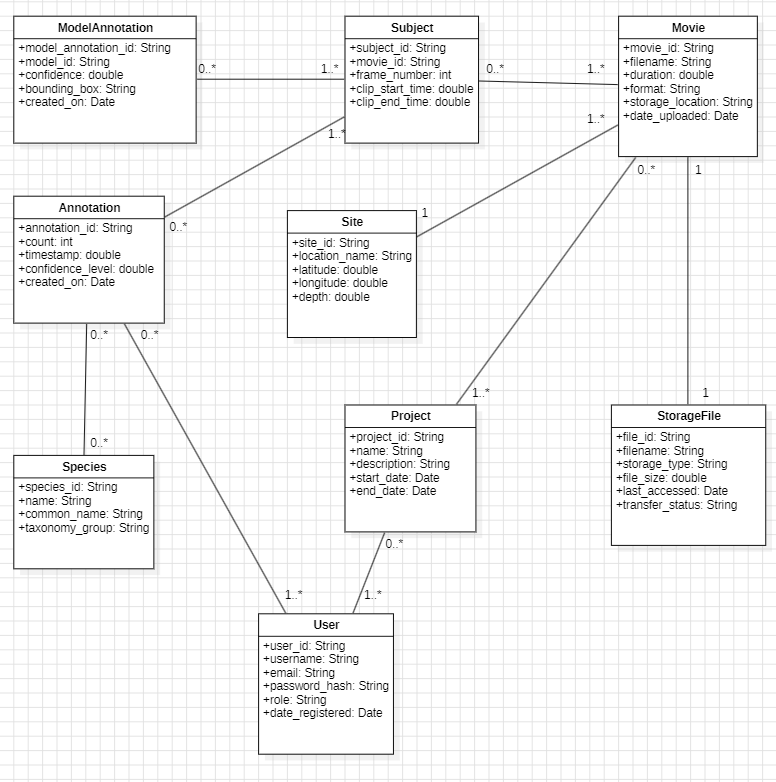
\includegraphics[width=1 \textwidth]{Figures/LogicalDatabase.png}
    \caption{Logical Database Diagram \label{Fig:Logical Database Diagram}}
\end{figure}

The logical database for the Koster Seafloor Observatory (KSO) efficiently manages user annotations, AI classifications, and ecological video data. It consists of interrelated tables that store movies, species, annotations, and storage files, ensuring structured data management. Users participate in projects, contributing to species classification on video clips (subjects), with AI models further refining these classifications. The database supports 1-to-1, 1-to-Many, and Many-to-Many relationships for efficient querying and retrieval. It enables seamless integration between citizen science efforts, machine learning automation, and marine research workflows.

\section{System Quality Attributes}
Dependability properties, Maintainability, and so on) in the order of priority with associated requirements. Usability, Performance and at least one additional quality attribute must be considered.

\subsection{Usability Requirements}
\begin{itemize}
    \item The system should be easy to install, configure, and operate, ensuring accessibility for researchers, citizen scientists, and other users with minimal technical expertise.
    \item The KSO platform should provide an intuitive and user-friendly interface for both data annotation and analysis, allowing seamless participation from citizen scientists.
    \item The system should support interactive data visualization tools that simplify the understanding and interpretation of marine ecological data.
    \item The interface should be accessible, incorporating features such as screen reader compatibility and adjustable font sizes to accommodate different user needs.
    \item The platform should automate repetitive tasks such as data pre-processing, annotation aggregation, and model training, reducing the manual workload for researchers.
    \item The system should provide real-time feedback and clear status indicators for data uploads, annotation progress, and model performance.
    \item The web interface should be aesthetically pleasing, engaging, and designed to enhance user motivation, especially for citizen scientists contributing to the classification process.
\end{itemize}

\subsection{Performance Requirements}
\begin{itemize}
    \item The system must support efficient handling and processing of large video datasets, ensuring smooth playback and frame extraction.
    \item Data transfer between storage, processing modules, and machine learning components should be optimized for minimal latency.
    \item The platform should leverage high-performance computing (HPC) resources to efficiently train machine learning models on large annotated datasets.
    \item The machine learning API should process requests in real-time, allowing researchers to obtain species identification results quickly.
    \item The system should handle concurrent user interactions, ensuring smooth annotation workflows on the citizen science platform.
\end{itemize}

\subsection{Reliability Requirements}
\begin{itemize}
    \item The system should ensure accurate and lossless transfer of video, annotation, and model prediction data between different modules.
    \item The machine learning model should produce consistent and reproducible results with a high confidence threshold (e.g., 0.7) to minimize errors in species identification.
    \item The database must maintain data integrity, ensuring that annotations from citizen scientists and model outputs are correctly stored and retrievable.
\end{itemize}

\subsection{Maintainability Requirements}
\begin{itemize}
    \item The system should follow a modular architecture, allowing independent updates and improvements to data management, citizen science, and machine learning components.
    \item Comprehensive documentation should be provided to facilitate future development, debugging, and system expansion.
    \item Version control systems (e.g., Git) must be used to track changes and enable rollbacks if necessary.
    \item Automated unit tests and integration tests should be developed to identify and resolve issues efficiently.
\end{itemize}

\subsection{Portability Requirements}
\begin{itemize}
    \item The KSO web platform should follow modern web standards to ensure compatibility with different devices and browsers.
    \item The machine learning models should be deployable across various computational environments, including cloud-based and on-premise HPC systems.
    \item The citizen science platform should be accessible from both desktop and mobile devices to maximize user engagement.
\end{itemize}

\section{Design Constraints}

The design of the Koster Seafloor Observatory is subject to the following constraints imposed by external factors, including regulatory requirements, official standards, and organizational limitations:

\begin{itemize}
    \item \textbf{Compliance with Data Standards}  
    \begin{itemize}
        \item The system follows the \textit{Darwin Core (DwC) Standards} \cite{anton2021kso} to ensure compatibility and interoperability with global biodiversity data repositories.
        \item Metadata associated with the underwater footage is regularly published in the \textit{Swedish National Data Archive}, requiring adherence to data formatting and archival standards.
    \end{itemize}
    
    \item \textbf{Open-Source Software Requirements}  
    \begin{itemize}
        \item The system is built entirely on \textit{open-source technologies}, which mandates that all software components, including machine learning models and citizen science tools, be freely available for modification and redistribution.
        \item The observatory must align with the principles of \textit{open science} and ensure that the tools and datasets can be accessed and reused by the broader research community.
    \end{itemize}

    \item \textbf{Regulatory and Ethical Compliance in Citizen Science}  
    \begin{itemize}
        \item The use of \textit{Zooniverse} for citizen science participation requires compliance with \textit{ethical guidelines} related to data privacy, user engagement, and volunteer contributions.
        \item Data collection involving human participants must adhere to the \textit{General Data Protection Regulation (GDPR)}, ensuring that personal data is handled securely and that no sensitive user information is collected.
    \end{itemize}

    \item \textbf{Hardware and Computational Constraints}  
    \begin{itemize}
        \item The system must operate within the specifications of the \textit{High Performance Computing (HPC) server}, which includes a \textit{GTX2080Ti GPU, Intel Core i9-9900 CPU, and 2GB DDR4 RAM} \cite{anton2021kso}.
        \item Machine learning algorithms must be optimized to function within these hardware limitations, balancing computational efficiency with model accuracy.
    \end{itemize}

    \item \textbf{Legal and Institutional Data Sharing Policies}  
    \begin{itemize}
        \item Data stored and processed by the observatory must comply with \textit{Swedish national regulations} on research data management and \textit{European Union directives on marine environmental protection}.
        \item Collaboration with institutions such as \textit{the University of Gothenburg and Chalmers University of Technology} requires alignment with their internal data storage, sharing, and security policies.
    \end{itemize}
\end{itemize}

\section{Supporting Information}
The \textbf{Koster Seafloor Observatory} is an \textbf{open-source} project designed to facilitate large-scale marine ecological research. The source code is publicly available on \textbf{GitHub}, allowing researchers, developers, and citizen scientists to explore and contribute to the project. Additionally, there are numerous open issues on the repository that require solutions, offering opportunities for contributors to support the project by developing and optimizing various modules.

Apart from contributing as a developer, individuals can participate in the project as \textbf{data annotators} through the \textbf{Zooniverse citizen science platform}. Volunteers can help classify marine species from underwater footage, improving the training dataset for machine learning models. Furthermore, researchers can validate machine learning outputs and provide expert classifications to enhance model accuracy.

The \textbf{Koster Seafloor Observatory} also offers an \textbf{Application Programming Interface (API)} and a \textbf{user-friendly web interface} for researchers to test machine learning models on new underwater footage. The system ensures compliance with \textbf{data-sharing standards}, including \textbf{Darwin Core (DwC)}, and follows \textbf{General Data Protection Regulation (GDPR)} guidelines to protect user privacy.

This supporting information is \textbf{not considered part of the core software requirements} but serves as valuable background material for users, contributors, and researchers engaging with the system.

